\section{Introduction}
\label{sec:introduction}

Modern Earth-observing (EO) satellites, while significantly more capable than those of the past, are still frequently operated with little autonomy: schedules are optimized on the ground, uplinked before execution, and then followed with limited ability to react to uncertain events in orbit.
This mode of operation is effective when target values are known or can be accurately forecasted, but is inefficient when planning under uncertainty.
Wildfires, volcanic eruptions, floods, storms, and other transient events can change where observations are valuable after a schedule is uplinked. The most common detractor of imaging is cloud cover---clouds occlude approximately 66\% of Earth's surface at any time~\citep{king_spatial_2013}, and if the objective is not to observe clouds, many scheduled imaging activities produce little value even when the pre-planned schedule is followed perfectly.

Dynamic targeting addresses this limitation by using onboard observations to re-optimize the schedule onboard.
We consider the case of a spacecraft with a secondary, body-fixed, wide-field instrument that observes upcoming targets, an onboard classifier estimates updated utility values, and the scheduler re-optimizes the schedule based on new information.
\figref{fig:conops} contrasts this onboard dynamic-tasking loop with conventional fixed-schedule execution.

\begin{figure}[t]
    \centering
    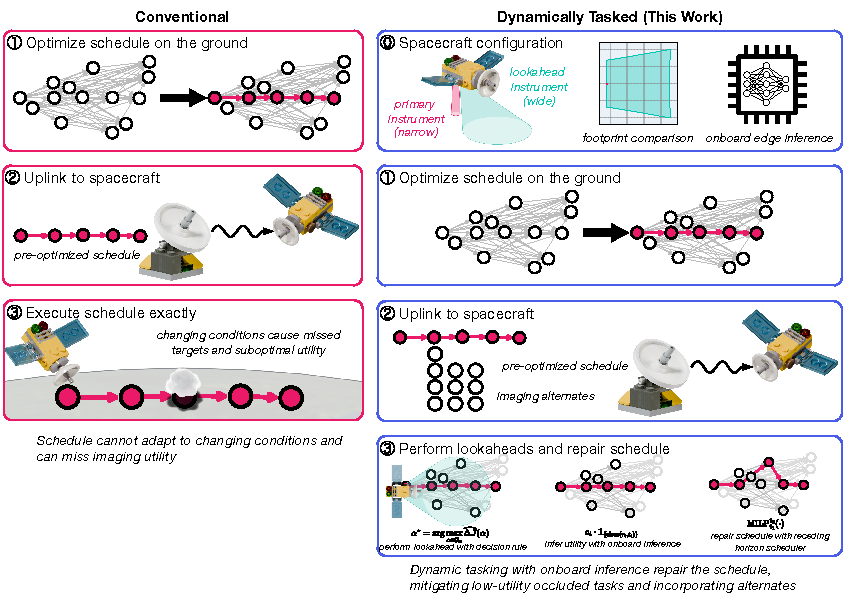
\includegraphics[width=\linewidth]{figures/dt_overview_new.pdf}
    \caption{Dynamic tasking concept of operations. \textbf{(left)} Conventional operations optimize and uplink a fixed schedule; when cloud state or task utility changes, the spacecraft may execute low-value collects. \textbf{(right)} In this work, a body-fixed wide-field lookahead instrument observes upcoming accesses, onboard inference updates candidate access utilities, and a receding-horizon scheduler repairs the local schedule before the primary imager commits.}
    \label{fig:conops}
\end{figure}

However, acquiring new information can come with its own costs---performing a lookahead can reveal viable alternative activities, but can consume slew time and may displace scheduled imaging, as well as inference time.
The utility of a lookahead action is therefore how much the schedule utility improves by, taking into account all gains and resource costs.

This makes body-fixed lookahead a value-of-information problem: the spacecraft is not simply choosing the next image, but choosing whether an attitude maneuver that gathers information will improve the downstream schedule enough to justify its cost.
Previous work often searches directly over lookahead actions or assumes a fixed observation strategy~\citep{kangaslahti_dynamic_2024, candela_dynamic_2022}, while in this work we frame dynamic tasking as decision analysis under flight-system constraints. We consider the bounding cases of a theoretical omniscient scheduler with perfect advance information, and a conventional scheduler executing a pre-planned schedule without deviation. The gap between them is therefore the expected value of perfect information (EVPI), and the gap closed by any dynamic tasking policy is its expected value of sample information (EVSI)~\citep{howard_information_1966, raiffa_applied_1968}.

Every contribution in this paper can be read through that lens: the systems analysis defines which information-gathering actions are physically available, the break-even utility rule decides whether those actions can repay their local schedule burden, and the timing and pointing rules maximize that margin over a schedule gap.

We make the following contributions:
\begin{enumerate}
    \item A \textbf{systems analysis} of body-fixed lookahead sensing for agile EO satellites, relating ConOps, field of view, geometry, and agility to the feasible information-gathering action space (\secref{sec:systems_analysis}).
    \item A \textbf{two-anchor renewal value model} for lookahead actions, plus a monotone break-even approximation that computes the maximum dead time each candidate pointing angle can tolerate and accepts the best angle only when that threshold exceeds the physical slew cost (\secref{sec:heuristic}).
    \item A \textbf{receding-horizon control loop} that combines camera projection, break-even pointing search, optimal maneuver timing, and local schedule repair into an onboard dynamic-tasking policy (\secref{sec:lookahead_policy}--\secref{sec:schedule_repair}).
\end{enumerate}

\paragraph{Paper organization.}
We review prior work on spacecraft scheduling, dynamic tasking, active perception, and sequential information acquisition (\secref{sec:background}), then analyze the spacecraft ConOps, request-to-access abstraction, field-of-view geometry, and agility constraints that reduce body-fixed lookahead tasking to a local onboard decision (\secref{sec:systems_analysis}). We then develop the break-even spacing rule, optimal timing and pitch search, and schedule repair loop that implement that decision (\secref{sec:method}). We close (\secref{sec:conclusion}) with the scope of the unit-utility, perfect-classification, and non-uniform request-utility assumptions.
